\documentclass[12pt, a4paper, oneside]{article}
\usepackage{CJKutf8}
\usepackage{amsmath, amsthm, amssymb, bm, color, framed, graphicx, hyperref, mathrsfs}
\usepackage{fancyhdr}
\usepackage{multicol}
\usepackage{mathtools}
\usepackage{gauss}
\usepackage[left=10mm, right=10mm, top=20mm, bottom=20mm]{geometry}
\pagestyle{fancy}
\fancyhf{}
\rhead{\begin{CJK}{UTF8}{gbsn}{计83 李天勤 2018080106}\end{CJK}}
\lhead{\begin{CJK}{UTF8}{gbsn}{高代线性代数作业7}\end{CJK}}
	

\title{\textbf{课程作业}}
\author{AkaCoder404}
\date{\today}
\newpage
\linespread{1.5}
\definecolor{shadecolor}{RGB}{241, 241, 255}
\newcounter{problemname}
\newenvironment{problem}{\begin{shaded}\stepcounter{problemname}\par\noindent\textbf{题目\arabic{problemname}. }}{\end{shaded}\par}
\newenvironment{solution}{\par\noindent\textbf{解答. }}{\par}
\newenvironment{note}{\par\noindent\textbf{题目\arabic{problemname}的注记. }}{\par}

% row operations
\newenvironment{sysmatrix}[1]
 {\left[\begin{array}{@{}#1@{}}}
 {\end{array}\right]}
\newcommand{\ro}[1]{%
  \xrightarrow{\mathmakebox[\rowidth]{#1}}%
}
\newlength{\rowidth} % row operation width

% kbordermatrix

% begin document  
\begin{document}
\begin{CJK}{UTF8}{gbsn}

% \maketitle
% \newpage
\section{Tangent vectors and Cotangent Vectors}

\setcounter{problemname}{0}
\begin{problem}
  For a symmetric positive-definite matrix $A$, and define $(v,w) = v^TAw$ \newline
\end{problem}

\begin{solution}
  1. Show that this is an inner product \newline
  To prove that the symmetric positive-definite matrix $A$ is an inner product, we need to prove for three cases
  $$ \begin{cases}
    1. \text{Bilinear} \\
    2. \text{Symmetric} \\
    3. \text{Positive-Definite}
  \end{cases}$$
  1. Bilinear
  $$ (kv, w) = (kv)^TAw = k(v^TAw) = k(v,w)$$ 
  $$ (v,kw) =v^TA(kw)=v^TA(kw)=kv^TAw=k(v,w)$$
  $$ (u+v,w) = (u+v)^TAw=u^TAw+v^TAw=(u,w)+(v,w) $$
  $$ (u, v+w) = u^TA(v+w) = u^TAv +u^TAw=(u,v)+(u,w)$$
  2. Symmetric
  $$ (u,w) = v^TAw$$
  $\because v^TAw$ is a scalar 
  $$ v^TAw = (v^Taw)^T=w^TA^Tv=(w,v)$$
  $$ \therefore (v,w) = (w,v) $$
  3. Positive Definite \newline
  $\because A$ is positive definite
  $$ (u,v)=v^TAv\geq 0,\forall v$$ and is equal to $0$ if $v=0$

\end{solution}

\begin{solution} 
  2. The Reiz map (inverse of the bra) from $V^*$ to $V$ would send a row vector $v^T$ to what? \newline
  The bra of $V$ is a linear map $\langle v, - \rangle$ such that $\begin{cases}
    V\mapsto R \\
    W\mapsto v^TAw
  \end{cases}$ \newline
  The bra map of $v$ is $\begin{cases}
     V \mapsto V^* \\
     v \mapsto v^TA
  \end{cases}$ \newline
  and since the Rieze map is the inverse of the bra map, the Riez Map is $\begin{cases}
    V^* \mapsto V \\
    v^TA \mapsto v
  \end{cases}$ \newline
  Let $v^TA=w^T \Rightarrow v = (w^TA^{-1})^T=A^{-T}w=A^{-1}w$ \newline
  $\therefore$ the Riez map is $w^T \mapsto A^{-1}w$, the Riez map sends the row vector $v^T$ to the column vector $A^{-1}v$
  \end{solution}

\begin{solution}
  3. The bra map from $V$ to $V*$ would send a vector $v$ to what? \newline
  The bra map sends vector $v$ to vector $v^TA$
\end{solution}

\begin{solution}
  4. The dual of the Riez map from $V*$ to $V$ would send a row vector $v^T$ to what? \newline
  Riez map $L:V*\rightarrow V$ \newline
  Let $\alpha \in V^*$ \newline
  Dual map of Riez map: $\alpha \rightarrow \alpha \circ L = L^*(\alpha)$ \newline
  $L^*$ sends $\alpha$ to $A^{-1}\alpha$ \newline
  \begin{figure}[h]
    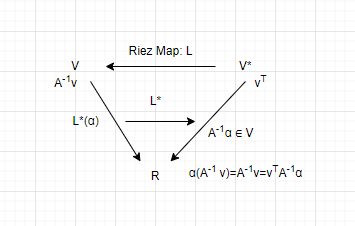
\includegraphics{image-20220513140213513.png}
    \centering
  \end{figure}
  $\therefore$ the dual map of Riez map sends $v^T to A^{-1}v$
\end{solution}

%--------------------------------------------------------------------
\begin{problem}
  What is a derivative?
\end{problem}

\begin{solution} 
  1. Constant functions in $V$ must be sent to zero by all derivations at any point. \newline
  Let $f$ be any constant function in $V$, dual vector $v_1\in V^*$ is derivation at $\vec{p}_1 \in M, \vec{p}$ is any point in $M$ \newline
  To prove, $v(f) = 0$, since $v_1$ is a derivation at $\vec{p} \in M$ \newline
  $\forall g \in V, \exists v_1(fg) = f(\vec{p})(g) + g(\vec{p})v_1(f)$  \newline
  WLOG, we can pick another constant $g \in V$, at $\vec{p}_2\in M$, there is a new derivation $v_2$ \newline
  \begin{equation}
    v_1(fg) = f(\vec{p}_1)v_1(g) + g(\vec{p}_1)v_1(f) = \text{const}_1 \cdot v_1(g) + \text{const}_2 \cdot v_1(f) 
  \end{equation}
  \begin{equation}
    v_2(fg) = f(\vec{p}_2)v_2(g) + g(\vec{p}_2)v_2(f) = \text{const}_1 \cdot v_2(g) + \text{const}_2 \cdot v_2(f) 
  \end{equation} 
  $$(1) - (2) = v_1(fg)-v_2(fg) = \text{const}_1\left[v_1(g)-v_2(g)\right] + \text{const}_2\left[v_1(f)-v_2(f)\right]$$
  $\because$ $v_1,v_2$ are dual vectors
  $$ (v_1-v_2)(fg) = \text{const}_1(v_1-v_2)(g) + \text{const}_2(v_1-v_2)(f) $$
  $$ \Rightarrow (v_1-v_2)(fg-\text{const}_1g-\text{const}_2f) = 0$$ 
  $$ \Rightarrow v_1 = v_2$$
  $ \because v_1 = v_2$, find a new function $t$ such that, $(1) \rightarrow (3), (2) \rightarrow (4)$
  \begin{equation}
    v_1(fg) = f(\vec{p}_1)v_1(t) + t(\vec{p}_1)v_1(f)
  \end{equation}
  \begin{equation}
    v_2(fg) = f(\vec{p}_2)v_2(t) + t(\vec{p}_2)v_2(f)
  \end{equation}
  $$ (3) - (4) \Rightarrow \left[ t(p_1) - t(p_2)\right]v(f)$$ 
  $$ v(f) = 0 $$
  $\therefore$ constant unctions in $V$ must be sent to zero by derivations at any point
\end{solution}

\begin{solution}
  2.  \newline
  Let $x-p_1=g_1$ be a function in $V$ \newline
  $\therefore$ we have 
  \begin{align}
    v((x-p_1)f) &= v(g_1f) \nonumber\\ 
    & =v(g_1)f(\vec{p})+v(f)g_1(\vec{p}) \nonumber\\
    & =f(\vec{p})v(x-p_1) + v(f)(p_1-p_1) \nonumber\\
    & =f(\vec{p})v(x-p_1) \nonumber\\
    & =f(\vec{p_1}\left[v(x)-v(p_1)\right]) \nonumber
  \end{align}
  $\because$ $p_1$ is a constant function, we know $v(p_1) = 0$
  $$ v(x-p_1)(f) = f(\vec{p})v(x)$$ 
  $\therefore$
  $$ v((y-p_2)f) = f(\vec{p})v(y) $$
  $$ v((z-p_3)f) = f(\vec{p})v(z) $$
\end{solution}

\begin{solution}
  3. \newline
  Since $a,b,c$ are nonnegative integers and $a+b+c>1$, they can't be 0 at the same time \newline
  Let $a \geq 1$, assume $f\vec{p} = (x-p_1)^{a-1}(y-p_2)^b(z-p_3)^c$ \newline
  Then $v((x-p_1)^a(y-p_2)^b(z-p_3)^c = v((x-p_1)f)$
  From problem 2, we know that 
  \begin{align}
     v(x-p_1)f &= f(\vec{p})v(x) \nonumber\\
     & = (p_1-p_1)^{a-1}(p_2-p_2)^b(p_3-p_3)^cv(x)  \nonumber\\
     & = 0^{a+b+C-1}v(x) \nonumber
  \end{align}
  $\because a+b+c-1>0, )^{a+b+c-1}v(x) = 0$ \newline
  $\therefore v((x-p_1)^a(x-p_2)^b(x-p_3)^c)=0$
\end{solution}

\begin{solution}
  4.\newline
  Since $f$ is an anyaltic function, we can first calculate the Taylor expansion of $f$ at $\vec{p} = \begin{bmatrix}
    p_1 \\ p_2 \\ p_3
  \end{bmatrix}$
  $$ f(x,y,z) = f(\vec{p}) + \frac{\partial f}{\partial x}(\vec{p})(x-p_1) + \frac{\partial f}{\partial y}(\vec{p})(y-p_2) + \frac{\partial f}{\partial z}(\vec{p})(z-p_3) + 0$$
  $$ = v(f(\vec{p}_1)) + \frac{\partial f}{\partial x}(\vec{p})v(x)-\frac{\partial f}{\partial x}(\vec{p})v(\vec{p}_1) + \frac{\partial f}{\partial y}(\vec{p})v(y)-\frac{\partial f}{\partial y}(\vec{p})v(\vec{p}_2) + \frac{\partial f}{\partial z}({\vec{p}})v(z) - \frac{\partial f}{\partial z}(\vec{p})v(\vec{p}_3)$$ 
  $$ = \frac{\partial f}{\partial x}(\vec{p})v(x)+\frac{\partial f}{\partial y}(\vec{p})v(y) + \frac{\partial f}{\partial z}(\vec{p})v(z)$$
\end{solution}

\begin{solution}
  5. \newline
  \begin{align}
    v(f) &= \frac{\partial f}{\partial x}(\vec{p})v(x)+\frac{\partial f}{\partial y}(\vec{p})v(y) + \frac{\partial f}{\partial z}(\vec{p})v(z) \nonumber \\
    & =\left[\frac{\partial f}{\partial x}, \frac{\partial f}{\partial y}, \frac{\partial f}{\partial z}\right](\vec{p})\begin{pmatrix}
      v(x) \\ v(y) \\ y(z)
    \end{pmatrix} \nonumber \\
    & =\nabla_v \rightarrow (f), \vec{v}=\begin{pmatrix}
      v(x) \\ v(y) \\ v(z)
    \end{pmatrix} \nonumber
  \end{align}
\end{solution}

%--------------------------------------------------------------------
\begin{problem}
  What is a vector field?
\end{problem}

\begin{solution} 
  1.  \newline
  $\because$ $x$ is a vector field
  $$ X_p(fg) = (X(fg)(\vec{p}))$$
  $$ X(fg) = fX(g) +gX(f)$$
  $$ X_{\vec{p}}(fg) = (X(fg))(\vec{p}) = \left[ fX(g) = gX(f)\right](\vec{p})$$
  $$ = (fX(g))(\vec{p}) + (gX(f))(\vec{p}) = f(\vec{p})X(g) + g(\vec{p})X(f))$$
  $\therefore$ $x$ follows the leibniz rule and is $x$ is a deivatation at $\vec{p}$ 
\end{solution}

\begin{solution}
  2. \newline
  $\forall \vec{p}$ $X(f)(\vec{p})=X_{\vec{p}}(f)$ \newline
  $X_{\vec{p}}$ is the derivation of any function at $\vec{p}$ \newline
  $X_{\vec{p}}$ evaluate the tiny change of $f$ with point $\vec{p}$'s velocity \newline
  $X_{\vec{p}}: V \mapsto R$ \newline
  $\partial f\vec{p}$ evaluates $X_{\vec{p}}$ to number $\mathbb{R}$ 
  $X_{\vec{p}}(f) = \partial f\vec{p}(X_{\vec{p}})$  \newline
  $\vec{p}$ is arbitrary point \newline
  $X(f) = \partial f(x)$ \newline
  $\partial f(x) = X(f)$

\end{solution}

\begin{solution}
  3. \newline
  Since $XY$ are a vector field
  $$X(fg) = fX(g)+gX(f)$$
  $$Y(fg) = fX(g)+gX(f)$$
  LHS = $(X\circ Y - Y\circ X)(fg) = X(fY(g) + gY(f)) - Y(fX(g) +gX(f))$ \newline
  $ = X(f)Y(g) + f(X\circ Y)(g) + X(g)Y(f) + g(X\circ Y)(f) - \left[Y(f)X(g)+f(Y\circ X)(g)+Y(g)X(f) + g(Y\circ X)(f)\right]$ \newline
  RHS = $(X\circ Y - Y\circ X)(g) + g(X\circ Y - Y\circ X)(f)$  \newline
  $ = f(X\circ Y)(g) - f(Y\circ X)(g) + g(X\circ Y)(f) - g(Y\circ X)(f)$ \newline
  Since 
  $$ X(f)Y(g) = Y(g)X(f)$$
  $$ Y(f)X(g) = X(g)Y(f)$$
  $$ \therefore LHS = RHS$$
  $\therefore X\circ Y - Y\circ X$ satisfies the leibniz rule \newline
  $\therefore X\circ Y - Y\circ X$ is always a vector field \newline
\end{solution}

\begin{solution}
  4.\newline
  If $A$,$B$ are skew-symmetric, then $A^T=-A, B^T=-B$
  \begin{align}
    (AB-BA)^T &= (AB)^T -(BA)^T = B^TA^T-A^TB^T \nonumber\\
    & =(-B)(-A) + (-A)(-B) \nonumber\\
    & =BA - AB \nonumber\\
    & =-(AB - BA) \nonumber
  \end{align}
  $\therefore$ $AB-BA$ is skew symmetric
\end{solution}


\end{CJK}
\end{document}